\documentclass[twoside]{book}

% Packages required by doxygen
\usepackage{fixltx2e}
\usepackage{calc}
\usepackage{doxygen}
\usepackage[export]{adjustbox} % also loads graphicx
\usepackage{graphicx}
\usepackage[utf8]{inputenc}
\usepackage{makeidx}
\usepackage{multicol}
\usepackage{multirow}
\PassOptionsToPackage{warn}{textcomp}
\usepackage{textcomp}
\usepackage[nointegrals]{wasysym}
\usepackage[table]{xcolor}

% NLS support packages
\usepackage{polski}
\usepackage[T1]{fontenc}

% Font selection
\usepackage[T1]{fontenc}
\usepackage[scaled=.90]{helvet}
\usepackage{courier}
\usepackage{amssymb}
\usepackage{sectsty}
\renewcommand{\familydefault}{\sfdefault}
\allsectionsfont{%
  \fontseries{bc}\selectfont%
  \color{darkgray}%
}
\renewcommand{\DoxyLabelFont}{%
  \fontseries{bc}\selectfont%
  \color{darkgray}%
}
\newcommand{\+}{\discretionary{\mbox{\scriptsize$\hookleftarrow$}}{}{}}

% Page & text layout
\usepackage{geometry}
\geometry{%
  a4paper,%
  top=2.5cm,%
  bottom=2.5cm,%
  left=2.5cm,%
  right=2.5cm%
}
\tolerance=750
\hfuzz=15pt
\hbadness=750
\setlength{\emergencystretch}{15pt}
\setlength{\parindent}{0cm}
\setlength{\parskip}{3ex plus 2ex minus 2ex}
\makeatletter
\renewcommand{\paragraph}{%
  \@startsection{paragraph}{4}{0ex}{-1.0ex}{1.0ex}{%
    \normalfont\normalsize\bfseries\SS@parafont%
  }%
}
\renewcommand{\subparagraph}{%
  \@startsection{subparagraph}{5}{0ex}{-1.0ex}{1.0ex}{%
    \normalfont\normalsize\bfseries\SS@subparafont%
  }%
}
\makeatother

% Headers & footers
\usepackage{fancyhdr}
\pagestyle{fancyplain}
\fancyhead[LE]{\fancyplain{}{\bfseries\thepage}}
\fancyhead[CE]{\fancyplain{}{}}
\fancyhead[RE]{\fancyplain{}{\bfseries\leftmark}}
\fancyhead[LO]{\fancyplain{}{\bfseries\rightmark}}
\fancyhead[CO]{\fancyplain{}{}}
\fancyhead[RO]{\fancyplain{}{\bfseries\thepage}}
\fancyfoot[LE]{\fancyplain{}{}}
\fancyfoot[CE]{\fancyplain{}{}}
\fancyfoot[RE]{\fancyplain{}{\bfseries\scriptsize Wygenerowano przez Doxygen }}
\fancyfoot[LO]{\fancyplain{}{\bfseries\scriptsize Wygenerowano przez Doxygen }}
\fancyfoot[CO]{\fancyplain{}{}}
\fancyfoot[RO]{\fancyplain{}{}}
\renewcommand{\footrulewidth}{0.4pt}
\renewcommand{\chaptermark}[1]{%
  \markboth{#1}{}%
}
\renewcommand{\sectionmark}[1]{%
  \markright{\thesection\ #1}%
}

% Indices & bibliography
\usepackage{natbib}
\usepackage[titles]{tocloft}
\setcounter{tocdepth}{3}
\setcounter{secnumdepth}{5}
\makeindex

% Hyperlinks (required, but should be loaded last)
\usepackage{ifpdf}
\ifpdf
  \usepackage[pdftex,pagebackref=true]{hyperref}
\else
  \usepackage[ps2pdf,pagebackref=true]{hyperref}
\fi
\hypersetup{%
  colorlinks=true,%
  linkcolor=blue,%
  citecolor=blue,%
  unicode%
}

% Custom commands
\newcommand{\clearemptydoublepage}{%
  \newpage{\pagestyle{empty}\cleardoublepage}%
}

\usepackage{caption}
\captionsetup{labelsep=space,justification=centering,font={bf},singlelinecheck=off,skip=4pt,position=top}

%===== C O N T E N T S =====

\begin{document}

% Titlepage & ToC
\hypersetup{pageanchor=false,
             bookmarksnumbered=true,
             pdfencoding=unicode
            }
\pagenumbering{roman}
\begin{titlepage}
\vspace*{7cm}
\begin{center}%
{\Large Aplikacja do optymalizacji nastaw regulatora silnika DC \\[1ex]\large 1.\+0 }\\
\vspace*{1cm}
{\large Wygenerowano przez Doxygen 1.8.11}\\
\end{center}
\end{titlepage}
\clearemptydoublepage
\tableofcontents
\clearemptydoublepage
\pagenumbering{arabic}
\hypersetup{pageanchor=true}

%--- Begin generated contents ---
\chapter{Indeks przestrzeni nazw}
\section{Lista przestrzeni nazw}
Tutaj znajdują się wszystkie udokumentowane przestrzenie nazw wraz z ich krótkimi opisami\+:\begin{DoxyCompactList}
\item\contentsline{section}{\hyperlink{namespaceGenop}{Genop} }{\pageref{d0/d54/namespaceGenop}}{}
\end{DoxyCompactList}

\chapter{Indeks hierarchiczny}
\section{Hierarchia klas}
Ta lista dziedziczenia posortowana jest z grubsza, choć nie całkowicie, alfabetycznie\+:\begin{DoxyCompactList}
\item Application\begin{DoxyCompactList}
\item \contentsline{section}{Genop.\+App}{\pageref{classGenop_1_1App}}{}
\end{DoxyCompactList}
\item \contentsline{section}{Genop.\+Controller}{\pageref{classGenop_1_1Controller}}{}
\item \contentsline{section}{Genop.\+Genetic\+Algorithm}{\pageref{classGenop_1_1GeneticAlgorithm}}{}
\item \contentsline{section}{Genop.\+Main\+View\+Model}{\pageref{classGenop_1_1MainViewModel}}{}
\item \contentsline{section}{Genop.\+P\+LC}{\pageref{classGenop_1_1PLC}}{}
\item \contentsline{section}{Genop.\+Simulator}{\pageref{classGenop_1_1Simulator}}{}
\item \contentsline{section}{Genop.\+Solver}{\pageref{classGenop_1_1Solver}}{}
\item Window\begin{DoxyCompactList}
\item \contentsline{section}{Genop.\+Main\+Window}{\pageref{classGenop_1_1MainWindow}}{}
\item \contentsline{section}{Genop.\+Window1}{\pageref{classGenop_1_1Window1}}{}
\end{DoxyCompactList}
\end{DoxyCompactList}

\chapter{Indeks klas}
\section{Lista klas}
Tutaj znajdują się klasy, struktury, unie i interfejsy wraz z ich krótkimi opisami\+:\begin{DoxyCompactList}
\item\contentsline{section}{\hyperlink{classGenop_1_1App}{Genop.\+App} \\*Logika interakcji dla klasy App.\+xaml }{\pageref{d7/db4/classGenop_1_1App}}{}
\item\contentsline{section}{\hyperlink{classGenop_1_1Controller}{Genop.\+Controller} }{\pageref{d7/da2/classGenop_1_1Controller}}{}
\item\contentsline{section}{\hyperlink{classGenop_1_1GeneticAlgorithm}{Genop.\+Genetic\+Algorithm} }{\pageref{d2/d5e/classGenop_1_1GeneticAlgorithm}}{}
\item\contentsline{section}{\hyperlink{classGenop_1_1MainViewModel}{Genop.\+Main\+View\+Model} }{\pageref{d5/d21/classGenop_1_1MainViewModel}}{}
\item\contentsline{section}{\hyperlink{classGenop_1_1MainWindow}{Genop.\+Main\+Window} \\*Logika interakcji dla klasy Main\+Window.\+xaml }{\pageref{d4/d4b/classGenop_1_1MainWindow}}{}
\item\contentsline{section}{\hyperlink{classGenop_1_1PLC}{Genop.\+P\+LC} }{\pageref{d7/d81/classGenop_1_1PLC}}{}
\item\contentsline{section}{\hyperlink{classGenop_1_1Simulator}{Genop.\+Simulator} }{\pageref{d7/dd0/classGenop_1_1Simulator}}{}
\item\contentsline{section}{\hyperlink{classGenop_1_1Solver}{Genop.\+Solver} }{\pageref{da/d16/classGenop_1_1Solver}}{}
\item\contentsline{section}{\hyperlink{classGenop_1_1Window1}{Genop.\+Window1} }{\pageref{d9/d56/classGenop_1_1Window1}}{}
\end{DoxyCompactList}

\chapter{Dokumentacja przestrzeni nazw}
\hypertarget{namespaceGenop}{}\section{Genop Namespace Reference}
\label{namespaceGenop}\index{Genop@{Genop}}
\subsection*{Classes}
\begin{DoxyCompactItemize}
\item 
class \hyperlink{classGenop_1_1App}{App}
\begin{DoxyCompactList}\small\item\em Logika interakcji dla klasy App.\+xaml \end{DoxyCompactList}\item 
class \hyperlink{classGenop_1_1Controller}{Controller}
\item 
class \hyperlink{classGenop_1_1GeneticAlgorithm}{Genetic\+Algorithm}
\item 
class \hyperlink{classGenop_1_1MainViewModel}{Main\+View\+Model}
\item 
class \hyperlink{classGenop_1_1MainWindow}{Main\+Window}
\begin{DoxyCompactList}\small\item\em Logika interakcji dla klasy Main\+Window.\+xaml \end{DoxyCompactList}\item 
class \hyperlink{classGenop_1_1PLC}{P\+LC}
\item 
class \hyperlink{classGenop_1_1Simulator}{Simulator}
\item 
class \hyperlink{classGenop_1_1Solver}{Solver}
\item 
class \hyperlink{classGenop_1_1Window1}{Window1}
\end{DoxyCompactItemize}

\chapter{Dokumentacja klas}
\hypertarget{classGenop_1_1App}{}\section{Dokumentacja klasy Genop.\+App}
\label{classGenop_1_1App}\index{Genop.\+App@{Genop.\+App}}


Logika interakcji dla klasy App.\+xaml  




Diagram dziedziczenia dla Genop.\+App
\nopagebreak
\begin{figure}[H]
\begin{center}
\leavevmode
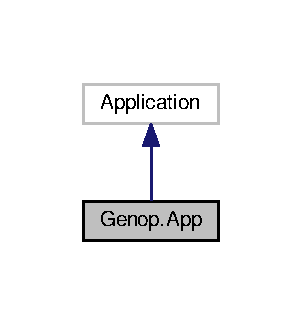
\includegraphics[width=145pt]{d1/d9b/classGenop_1_1App__inherit__graph}
\end{center}
\end{figure}


Diagram współpracy dla Genop.\+App\+:
\nopagebreak
\begin{figure}[H]
\begin{center}
\leavevmode
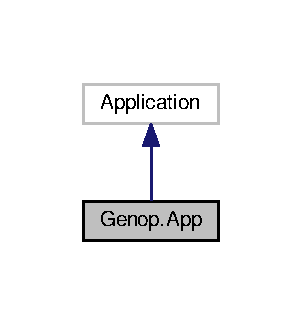
\includegraphics[width=145pt]{dd/de4/classGenop_1_1App__coll__graph}
\end{center}
\end{figure}


\subsection{Opis szczegółowy}
Logika interakcji dla klasy App.\+xaml 



Dokumentacja dla tej klasy została wygenerowana z pliku\+:\begin{DoxyCompactItemize}
\item 
/home/paceu/\+P\+O\+S/\+R\+E\+P\+O1/\+Genetic\+Optimization/\+Genop/\+Genop/App.\+xaml.\+cs\end{DoxyCompactItemize}

\hypertarget{classGenop_1_1Controller}{}\section{Genop.\+Controller Class Reference}
\label{classGenop_1_1Controller}\index{Genop.\+Controller@{Genop.\+Controller}}
\subsection*{Public Member Functions}
\begin{DoxyCompactItemize}
\item 
double {\bfseries Calculate\+Output} (double error, double dt)\hypertarget{classGenop_1_1Controller_ae5fd8ff66bb482c175bd02aa2366a336}{}\label{classGenop_1_1Controller_ae5fd8ff66bb482c175bd02aa2366a336}

\end{DoxyCompactItemize}


The documentation for this class was generated from the following file\+:\begin{DoxyCompactItemize}
\item 
Controller.\+cs\end{DoxyCompactItemize}

\hypertarget{classGenop_1_1GeneticAlgorithm}{}\section{Dokumentacja klasy Genop.\+Genetic\+Algorithm}
\label{classGenop_1_1GeneticAlgorithm}\index{Genop.\+Genetic\+Algorithm@{Genop.\+Genetic\+Algorithm}}


Dokumentacja dla tej klasy została wygenerowana z pliku\+:\begin{DoxyCompactItemize}
\item 
/home/paceu/\+P\+O\+S/\+R\+E\+P\+O1/\+Genetic\+Optimization/\+Genop/\+Genop/Genetic\+Algorithm.\+cs\end{DoxyCompactItemize}

\hypertarget{classGenop_1_1MainViewModel}{}\section{Dokumentacja klasy Genop.\+Main\+View\+Model}
\label{classGenop_1_1MainViewModel}\index{Genop.\+Main\+View\+Model@{Genop.\+Main\+View\+Model}}
\subsection*{Właściwości}
\begin{DoxyCompactItemize}
\item 
Plot\+Model {\bfseries Model}\hspace{0.3cm}{\ttfamily  \mbox{[}get\mbox{]}}\hypertarget{classGenop_1_1MainViewModel_aa9c636994e88a30f28caaee2435b2423}{}\label{classGenop_1_1MainViewModel_aa9c636994e88a30f28caaee2435b2423}

\end{DoxyCompactItemize}


Dokumentacja dla tej klasy została wygenerowana z pliku\+:\begin{DoxyCompactItemize}
\item 
Window1.\+xaml.\+cs\end{DoxyCompactItemize}

\hypertarget{classGenop_1_1MainWindow}{}\section{Genop.\+Main\+Window Class Reference}
\label{classGenop_1_1MainWindow}\index{Genop.\+Main\+Window@{Genop.\+Main\+Window}}


Logika interakcji dla klasy Main\+Window.\+xaml  




Inheritance diagram for Genop.\+Main\+Window\+:
\nopagebreak
\begin{figure}[H]
\begin{center}
\leavevmode
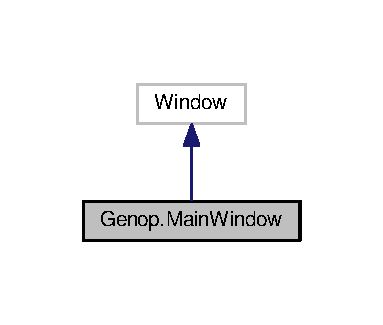
\includegraphics[width=184pt]{classGenop_1_1MainWindow__inherit__graph}
\end{center}
\end{figure}


Collaboration diagram for Genop.\+Main\+Window\+:
\nopagebreak
\begin{figure}[H]
\begin{center}
\leavevmode
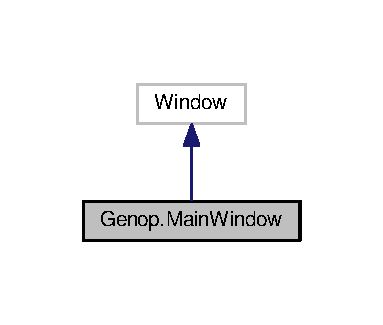
\includegraphics[width=184pt]{classGenop_1_1MainWindow__coll__graph}
\end{center}
\end{figure}


\subsection{Detailed Description}
Logika interakcji dla klasy Main\+Window.\+xaml 



The documentation for this class was generated from the following file\+:\begin{DoxyCompactItemize}
\item 
Main\+Window.\+xaml.\+cs\end{DoxyCompactItemize}

\hypertarget{classGenop_1_1PLC}{}\section{Dokumentacja klasy Genop.\+P\+LC}
\label{classGenop_1_1PLC}\index{Genop.\+P\+LC@{Genop.\+P\+LC}}
\subsection*{Metody publiczne}
\begin{DoxyCompactItemize}
\item 
double\mbox{[}$\,$\mbox{]} {\bfseries Auto\+Identyfication} ()\hypertarget{classGenop_1_1PLC_afa849d2eba7ea7ba9f2c36364e069c45}{}\label{classGenop_1_1PLC_afa849d2eba7ea7ba9f2c36364e069c45}

\end{DoxyCompactItemize}


Dokumentacja dla tej klasy została wygenerowana z pliku\+:\begin{DoxyCompactItemize}
\item 
/home/paceu/\+P\+O\+S/\+R\+E\+P\+O1/\+Genetic\+Optimization/\+Genop/\+Genop/P\+L\+C.\+cs\end{DoxyCompactItemize}

\hypertarget{classGenop_1_1Simulator}{}\section{Genop.\+Simulator Class Reference}
\label{classGenop_1_1Simulator}\index{Genop.\+Simulator@{Genop.\+Simulator}}


Collaboration diagram for Genop.\+Simulator\+:
\nopagebreak
\begin{figure}[H]
\begin{center}
\leavevmode
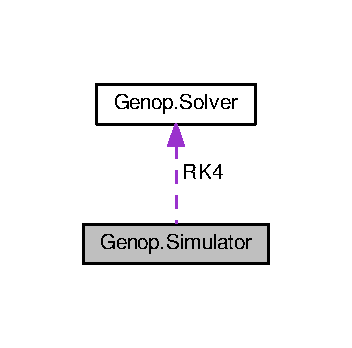
\includegraphics[width=169pt]{classGenop_1_1Simulator__coll__graph}
\end{center}
\end{figure}
\subsection*{Public Member Functions}
\begin{DoxyCompactItemize}
\item 
void {\bfseries Get\+User\+Parameters} (double\mbox{[}$\,$\mbox{]} object\+Parameters)\hypertarget{classGenop_1_1Simulator_a4bed492f372adb3bfb577a5caf7a143a}{}\label{classGenop_1_1Simulator_a4bed492f372adb3bfb577a5caf7a143a}

\item 
double\mbox{[}$\,$\mbox{]} {\bfseries Simulate} (int number\+Of\+Probes, double time\+Step=0.\+001)\hypertarget{classGenop_1_1Simulator_ac3228946a174bafc232038ee2f74141c}{}\label{classGenop_1_1Simulator_ac3228946a174bafc232038ee2f74141c}

\end{DoxyCompactItemize}
\subsection*{Public Attributes}
\begin{DoxyCompactItemize}
\item 
\hyperlink{classGenop_1_1Solver}{Solver} {\bfseries R\+K4} = new \hyperlink{classGenop_1_1Solver}{Solver}()\hypertarget{classGenop_1_1Simulator_af3757fb33e92dbf3a883156d7289d6ec}{}\label{classGenop_1_1Simulator_af3757fb33e92dbf3a883156d7289d6ec}

\end{DoxyCompactItemize}


The documentation for this class was generated from the following file\+:\begin{DoxyCompactItemize}
\item 
Simulator.\+cs\end{DoxyCompactItemize}

\hypertarget{classGenop_1_1Solver}{}\section{Dokumentacja klasy Genop.\+Solver}
\label{classGenop_1_1Solver}\index{Genop.\+Solver@{Genop.\+Solver}}
\subsection*{Metody publiczne}
\begin{DoxyCompactItemize}
\item 
double {\bfseries calculate\+Rotor\+Current} (double x1, double x2, double U)\hypertarget{classGenop_1_1Solver_a284e2f18385857212e8a2cc38f14c155}{}\label{classGenop_1_1Solver_a284e2f18385857212e8a2cc38f14c155}

\item 
double {\bfseries calculate\+Angular\+Velocity} (double x1, double x2, double Tl=0)\hypertarget{classGenop_1_1Solver_ac40d9b2668f551bfc3c4e2b5f054012a}{}\label{classGenop_1_1Solver_ac40d9b2668f551bfc3c4e2b5f054012a}

\item 
double\mbox{[}$\,$\mbox{]} {\bfseries Calculate\+Next\+Step} (double U, double h=0.\+001)\hypertarget{classGenop_1_1Solver_ad03d8a897aa8db437cc46b54872e021d}{}\label{classGenop_1_1Solver_ad03d8a897aa8db437cc46b54872e021d}

\end{DoxyCompactItemize}
\subsection*{Atrybuty publiczne}
\begin{DoxyCompactItemize}
\item 
double {\bfseries La}\hypertarget{classGenop_1_1Solver_a6d1c056f0852c4ff60804fb5ffee2bcc}{}\label{classGenop_1_1Solver_a6d1c056f0852c4ff60804fb5ffee2bcc}

\item 
double {\bfseries Lf}\hypertarget{classGenop_1_1Solver_a8f9b37a235ba4f5d508ed939ca920a6d}{}\label{classGenop_1_1Solver_a8f9b37a235ba4f5d508ed939ca920a6d}

\item 
double {\bfseries Laf}\hypertarget{classGenop_1_1Solver_a94d64291faa7206ef19499dc468afc5e}{}\label{classGenop_1_1Solver_a94d64291faa7206ef19499dc468afc5e}

\item 
double {\bfseries T}\hypertarget{classGenop_1_1Solver_a4b843e4fbca0a421ece8fffb4f59236f}{}\label{classGenop_1_1Solver_a4b843e4fbca0a421ece8fffb4f59236f}

\item 
double\mbox{[}$\,$\mbox{]} {\bfseries x} = new double\mbox{[}2\mbox{]}\hypertarget{classGenop_1_1Solver_ac15052491c6a89063cf8c6b679552c3b}{}\label{classGenop_1_1Solver_ac15052491c6a89063cf8c6b679552c3b}

\end{DoxyCompactItemize}


Dokumentacja dla tej klasy została wygenerowana z pliku\+:\begin{DoxyCompactItemize}
\item 
Solver.\+cs\end{DoxyCompactItemize}

\hypertarget{classGenop_1_1Window1}{}\section{Dokumentacja klasy Genop.\+Window1}
\label{classGenop_1_1Window1}\index{Genop.\+Window1@{Genop.\+Window1}}


Diagram dziedziczenia dla Genop.\+Window1
\nopagebreak
\begin{figure}[H]
\begin{center}
\leavevmode
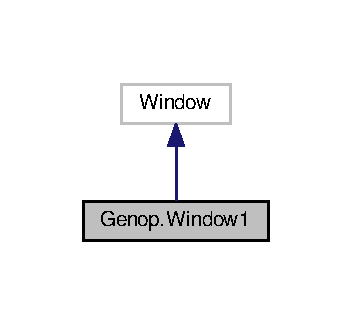
\includegraphics[width=169pt]{dc/de5/classGenop_1_1Window1__inherit__graph}
\end{center}
\end{figure}


Diagram współpracy dla Genop.\+Window1\+:
\nopagebreak
\begin{figure}[H]
\begin{center}
\leavevmode
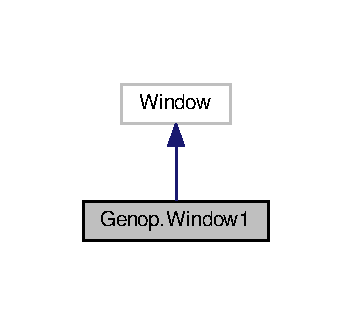
\includegraphics[width=169pt]{d7/d3b/classGenop_1_1Window1__coll__graph}
\end{center}
\end{figure}


Dokumentacja dla tej klasy została wygenerowana z pliku\+:\begin{DoxyCompactItemize}
\item 
/home/paceu/\+P\+O\+S/\+R\+E\+P\+O1/\+Genetic\+Optimization/\+Genop/\+Genop/Window1.\+xaml.\+cs\end{DoxyCompactItemize}

%--- End generated contents ---

% Index
\backmatter
\newpage
\phantomsection
\clearemptydoublepage
\addcontentsline{toc}{chapter}{Indeks}
\printindex

\end{document}
